\subsection{Versuchsaufbau}
\label{sec:Versuchsaufbau}

Der verwendete Aufbau ist in Abbildung~\ref{fig:aufbau} dargestellt. Alle Bauteile sind auf einer Schiene angebracht, sodass die
relativen Abstände variiert werden können. Bevor relevante Merkmale des Lasers vermessen werden können, ist eine
Justage des Aufbaus notwendig. Hierzu wird ein Justierlaser und zwei Beugungsblenden verwendet.
Nach erfolgreicher Vorjustage wird am Laserrohr eine Hochspanung
angelegt, die die notwendige Gasentladung hervorruft. Durch Justierschrauben an den konfokalen Resonatorspiegeln (Radius jeweils $\SI{1.4}{\meter}$)
und dem Laserrohr werden die Elemente so nachjustiert, dass die optischen Achsen aufeinander liegen und der Laser anfängt zu leuchten.
Zur Intensitätsmessung wird eine Photodiode verwendet, die auf der Strahlachse des Laser positioniert ist.
\begin{figure}
  \centering
  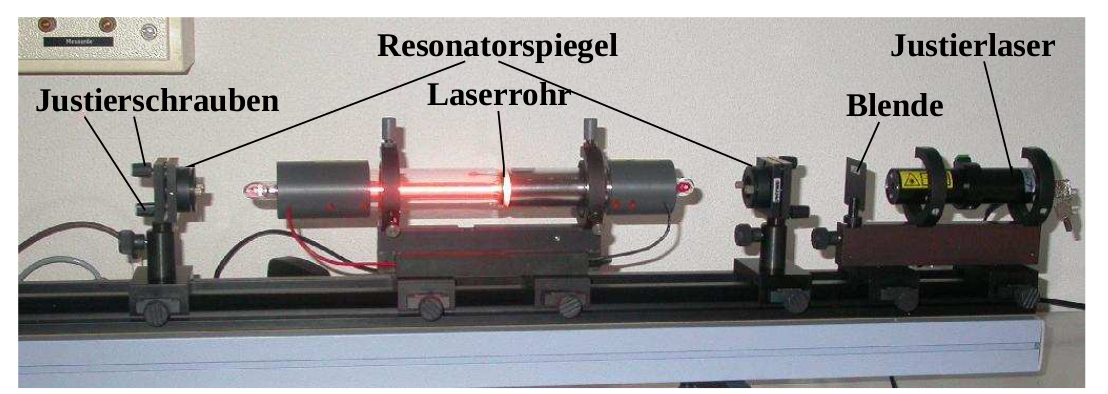
\includegraphics[width=0.99\columnwidth]{pictures/aufbau.png}
  \caption{Darstellung des Versuchsaufbaus.~\cite{Anleitung}}
  \label{fig:aufbau}
\end{figure}
